% When using TeXShop on the Mac, let it know the root document. The following must be one of the first 20 lines.
% !TEX root = ../design.tex

\chapter[Decision trees]{Decision Trees: Classification and Regression}
\begin{moduleinfo}
\item[Authors] {Rahul Iyer and Liquan Pei}
\item[History]
    \begin{modulehistory}
            \item[v0.2] Parallelism
            \item[v0.1] Initial version: introduction, theory, and interface
    \end{modulehistory}
\end{moduleinfo}

% Abstract. What is the problem we want to solve?
\section{Introduction} % (fold)
\label{sec:introduction}


\emph{Notes, examples and figures in this section are borrowed from
\cite{hastie2008statisticallearning} and \cite{james2013statisticallearning}}.


Tree-based methods for regression and classification involve stratifying or
segmenting the predictor space into a number of simple regions. In order to make
a prediction for a given observation, we typically use the mean or the mode of
the training observations in the region to which it belongs. Since the set of
splitting rules used to segment the predictor space can be summarized in a tree,
these types of approaches are known as decision tree methods. Tree-based methods
are simple and useful for interpretation. However, they typically are not
competitive with the best supervised learning approaches, in terms of
prediction accuracy. The results from multiple decision tree are usually combined
to yield a single consensus prediction often resulting in dramatic improvements
in prediction accuracy, at the expense of some loss in interpretation.

\subsection{Basics of Decision Trees} % (fold)
\label{sub:basics_of_decision_trees}
In order to motivate tree methods, we begin with a simple example.

\begin{figure}[h!tb]
    \begin{center}
        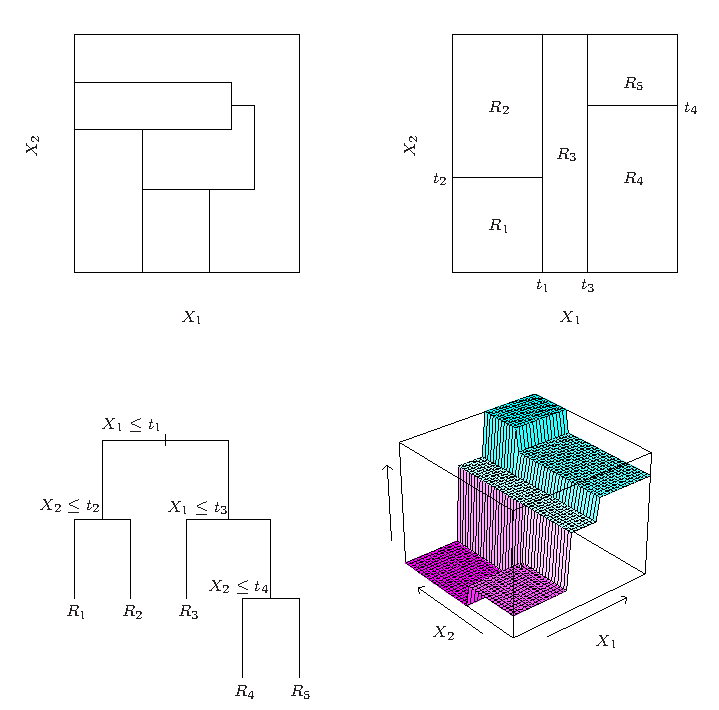
\includegraphics[width=0.8\textwidth]{figures/basics_decision_tree}
    \end{center}
    \caption{(Figure from \cite{hastie2008statisticallearning}.)
    Top right panel shows a partition of a two-dimensional
    feature space by recursive binary splitting, applied to
    some arbitrary data. Top left panel shows a general partition that cannot be
    obtained from recursive binary splitting. Bottom left panel shows the tree
    corresponding to the partition in the top right panel, and a perspective
    plot of the prediction surface appears in the bottom right panel.}
    \label{fig:basics_decision_tree}
\end{figure}
Let's consider a regression problem with continuous response $Y$ and inputs
$X_1$ and $X_2$, each taking values in the unit interval. The top left panel of
Figure~\ref{fig:basics_decision_tree} shows a partition of the feature space by
lines that are parallel to the coordinate axes. In each partition element we can
model $Y$ with a different constant. However, there is a problem: although each
partitioning line has a simple description like $X_1 = c$, some of the resulting
regions are complicated to describe.

To simplify matters, we restrict attention to recursive binary partitions like
that in the top right panel of Figure~\ref{fig:basics_decision_tree}. We first
split the space into two regions, and model the response by the mean of $Y$ in
each region. We choose the variable and split-point to achieve the best fit.
Then one or both of these regions are split into two more regions, and this
process is continued, until some stopping rule is applied. For example, in the
top right panel of Figure~\ref{fig:basics_decision_tree}, we first split at
$X_1 = t1$. Then the region $X1 \le t1$ is split at $X2 = t2$ and the region
$X1 > t1$ is split at $X1 = t3$. Finally,the region $X1 > t3$ is split at
$X2 = t4$. The result of this process is a partition into the five
regions $R_1, R_2, \ldots, R_5$ shown in the figure. The corresponding regression
model predicts $Y$ with a constant $c_m$ in region $R_m$, that is,
$$
    f(X) = \sum_{m=1}^{5} c_m I{(X_1, X_2) \in R_m}.
$$

This same model can be represented by the binary tree in the bottom left panel
of Figure~\ref{fig:basics_decision_tree}. The full dataset sits at the top of
the tree. Observations satisfying the condition at each junction are assigned to
the left branch, and the others to the right branch. The terminal nodes or
leaves of the tree correspond to the regions $R_1, R_2, \ldots, R_5$. The bottom
right panel is a perspective plot of the regression surface from this model.

\paragraph{Prediction via Stratification of the Feature Space:}

We now discuss the process of building a regression tree. Roughly speaking,
there are two steps.
\begin{enumerate}
    \item We divide the predictor space - that is, the set of possible values for
$X1, X2, \ldots, Xp$ into $J$ distinct and non-overlapping regions, $R_1, R_2,
\ldots, R_J$.
    \item For every observation that falls into the region $R_j$, we make the same
    prediction, which is simply the mean of the response values for the training
    observations in $R_j$.
\end{enumerate}

\paragraph{Advantages of using tree-based models:}

\begin{enumerate}
    \item Trees are very easy to explain to people.
    \item Some believe that decision trees more closely mirror human decision-making.
    \item Trees can be displayed graphically, and are easily interpreted even by a non-expert.
    \item Trees can easily handle qualitative predictors without the need to create dummy variables.
\end{enumerate}
% subsection basics_of_decision_trees (end)

\subsection{Trees Versus Linear Models} % (fold)
\label{sub:trees_versus_linear_models}
\begin{figure}[h!tb]
    \begin{center}
        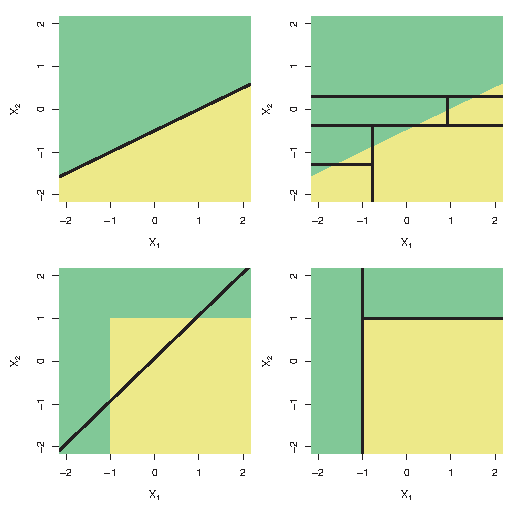
\includegraphics[width=0.7\textwidth]{figures/decision_tree_linear_model}
    \end{center}
    \caption{(Figure from \cite{james2013statisticallearning}.)
Top Row: A two-dimensional classification example in which the true decision
boundary is linear, and is indicated by the shaded regions. A classical approach
that assumes a linear boundary (left) will outperform a decision tree that
performs splits parallel to the axes (right). Bottom Row: Here the true decision
boundary is non-linear. Here a linear model is unable to capture the true
decision boundary (left), whereas a decision tree is successful (right).}
    \label{fig:decision_trees_linear_models}
\end{figure}

Regression and classification trees have a very different flavor from the more
classical approaches for regression presented in \ref{chap:regression}.
In particular, linear regression assumes a model of the form
$$
        f(X) = \beta_0 + \sum_{j=1}^{p} X_j \beta_j,
$$
whereas regression trees assume a model of the form
$$
        f(X) = \sum_{m=1}^{M} c_m \cdot 1_{X \in R_m}
$$
where $R_1, \ldots, R_M$ represent a partition of feature space.
The efficacy of the two models depend on the problem at hand, as illustrated by
Figure~\ref{fig:decision_trees_linear_models}
% subsection trees_versus_linear_models (end)
% section introduction (end)

\section{Interface} % (fold)
\label{sec:interface}
The interface of the decision tree functionality includes two functions,
\texttt{tree\_train} and \texttt{tree\_predict}, described below.

\subsection{Training} % (fold)
\label{sub:training}
\begin{sql}
    SELECT tree_train(
            split_criterion,
            training_table_name,
            output_table_name,
            id_col_name,
            list_of_features,
            dependent_variable,
            list_of_features_to_exclude,
            grouping_cols,
            weights,
            max_depth,
            min_split,
            min_bucket,
            cp,
            verbose
    )
\end{sql}

\paragraph{Arguments:}

\begin{itemize}
    % \item \emph{training\_algorithm}: Can be either `c4.5' or `cart'
    \item \emph{split\_criterion}: Various options to compute the feature
    to split a node. Available options are `gini', `cross-entropy', and
    `misclassification'.
    The ``cart'' algorithm provides an additional option of `mse'.
    \item \emph{training\_table\_name}: Name of the table containing data.
    \item \emph{output\_table\_name}: Name of the table to output the model.
    \item \emph{id\_col\_name}: Name of column containing the id information in training data.
    \item \emph{dependent\_variable}: Name of the column that contains the
    output for training. Boolean, integer and text are considered classification
    outputs, while float values are considered regression outputs.
    \item \emph{list\_of\_features}: List of column names (comma-separated string)
    to use as predictors. Can also be a `*' implying all columns are to be used
    as predictors (except the ones included in the next argument). Boolean, integer, and
    text columns are considered categorical columns.
    \item \emph{list\_of\_features\_to\_exclude}: OPTIONAL. List of column names (comma-separated string)
    to exlude from the predictors list.
    \item \emph{grouping\_cols}: OPTIONAL. List of column names (comma-separated string) to group
    the data by. This will lead to creating multiple decision trees, one for each group.
    \item \emph{weights}: OPTIONAL. Column name containing weights for each observation.
    \item \emph{max\_depth}: OPTIONAL (Default = 10). Set the maximum depth of
    any node of the final tree, with the root node counted as depth 0.
    \item \emph{min\_split}: OPTIONAL (Default = 20). Minimum number of observations that
    must exist in a node for a split to be attempted.
    \item \emph{min\_bucket}: OPTIONAL (Default = minsplit/3). Minimum number of observations
    in any terminal node. If only one of minbucket or minsplit is specified,
    minsplit is set to minbucket*3 or minbucket to minsplit/3, as appropriate.
    % \item \emph{use\_surrogate}: OPTIONAL (Default = 0) Use of surrogates in splitting process.
    %     \begin{enumerate}
    %         \setcounter{enumi}{0}
    %         \item An observation with a missing value for the primary split rule
    %         is not sent further down the tree.
    %         \item
    %         \item If all surrogates are missing, then send the observation in the majority direction.
    %     \end{enumerate}
    % \item \emph{surrogate\_style}: OPTIONAL (Default = 0)
    %     \begin{enumerate}
    %         \setcounter{enumi}{0}
    %         \item Use total number of correct classification for a potential surrogate variable
    %         \item Use the percent correct, calculated over the non-missing values of the surrogate
    %     \end{enumerate}
    % \item \emph{max\_surrogate}: OPTIONAL (Default = 0)
    % The number of surrogate splits retained in the output. If this is set to zero the compute time will be reduced.
    % \item \emph{max\_compete}: OPTIONAL (Default = 0) Number of competitor splits
    % retained in the output. It is useful to know not just which split was chosen,
    % but which variable came in second, third, etc.
    \item \emph{n\_bins}: OPTIONAL (Default = 100) Number of bins to use during binning.
    Continuous-valued features are binned into discrete bins (per the quartile values)
    to compute split boundaries. This global parameter is used to compute the resolution of the bins. Higher number of bins will lead to higher processing time.
    \item \emph{cp}: OPTIONAL (Default = 0.01)
        % For `c4.5', a statistical confidence interval of the re-substitution error;
        % for `cart',
        A complexity parameter that determines that a split is attempted only if it
        decreases the overall lack of fit by a factor of `cp'.
    \item \emph{n\_folds}: OPTIONAL (Default = 10) Number of cross-validation folds
    \item \emph{verbose}: OPTIONAL (Default = False) Prints status information
     on the splits performed and any other information useful for debugging.
\end{itemize}
% subsection training (end)

\subsection{Prediction} % (fold)
\label{sub:prediction}
\begin{sql}
    SELECT tree_predict(
            tree_model,
            new_data_table,
            output_table,
            type
    )
\end{sql}

\paragraph{Arguments:}

\begin{itemize}
    \item \emph{tree\_model}: Name of the table containing the decision tree model.
    \item \emph{new\_data\_table}: Name of table containing prediction data.
    \item \emph{output\_table}: Name of table to output prediction results.
    \item \emph{type}: OPTIONAL (Default = `response'). For regression trees,
    `response', implies output is the predicted value. For classification trees,
    this can be `response', giving the classification prediction as output, or
    `prob', giving the class probabilities as output
    (for two classes, only a single probability value is output that corresponds
    to the first class when the two classes are sorted by name;
    in case of more than two classes, an array of class probabilities
    (a probability of each class) is output).
\end{itemize}
% subsection prediction (end)
% section interface (end)
\section{CART} % (fold)
\label{sec:cart}
CART stands for Classification and Regression Trees (\cite{breiman1984cart}). It
is characterized by the fact that it constructs binary trees, namely each
internal node has exactly two outgoing edges. The splits can be selected using
any of the impurity metrics criteria and the obtained tree is pruned by
cost-complexity pruning.

\subsection{Impurity metrics} % (fold)
\label{sub:impurity_metrics}
\begin{figure}[h!tb]
    \begin{center}
        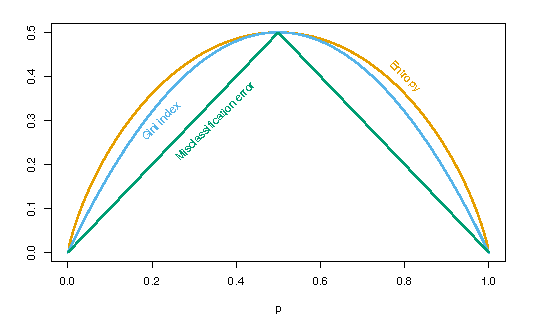
\includegraphics[width=0.65\textwidth]{figures/impurity_measures}
    \end{center}
    \caption{(Figure obtained from \cite{hastie2008statisticallearning})
Node impurity measures for two-class classification, as a function of the
proportion $p$ in class 2. Cross-entropy has been scaled to pass through (0.5, 0.5).}
    \label{fig:impurity_measures}
\end{figure}

The measures developed for selecting the best split are often based on the
degree of impurity of the child nodes. The smaller the degree of impurity,
the more skewed the class distribution.  For example, a node with class
distribution $(0, 1)$ has zero impurity, whereas a node with uniform class
distribution $(0.5, 0.5)$ has the highest impurity. Examples of impurity
measures include

\begin{itemize}
    \item Cross-entropy: $- \displaystyle \sum_{i=1}^{C}p(i|A)\log_2 p(i|A)$
    \item Gini: $1 - \displaystyle \sum_{i=1}^{C} \left(p(i|A)\right)^2$
    \item Classification error: $1 - \displaystyle \max_{i \in 1\ldots C} p(i|A)$,
\end{itemize}
where $C$ is the number of classes and $p(i|A)$ denotes the proportion of records
belonging to class $i$ at a given node $A$.

Figure~\ref{fig:impurity_measures} compares the values of the impurity measures
for binary classification problems. p refers to the fraction of records that
belong to one of the two classes. Observe that all three measures attain their
maximum value when the class distribution is uniform (i.e., when p = 0.5). The
minimum values for the measures are attained when all the records belong to the
same class (i.e., when p equals 0 or 1).

A split for a node is computed by how much `impurity' is reduced by that split.
For example, if we use the Gini index for selecting the split, we obtain the best
binary split ($D_1$ and $D_2$) that maximizes the Gini gain as,
$$
    G_\text{gini}(D; D_1, D_2)= g(D) - \left( \frac{|D_1|}{|D|} g(D_1) +
                                              \frac{|D_2|}{|D|} g(D_2) \right),
$$ where $g(D)$ is the Gini impurity metric.

For ordered, continuous attributes, we create splits of the form $X_i < v$,
where $X_i$ is an attribute and $v$ is a value in the domain of $X_i$, allowing
possibly infinite such splits. To reduce the computational load, we compute
quantile boundaries of the attribute and test for splits on these boundary
values.

For categorical attributes, we create splits of the form
$X_i \in \{v_1, v_2, v_3, \ldots\}$, where $\{v_1, v_2, v_3, \ldots\}$ is
a subset of all possible values of the categorical attribute. For ordered,
categorical attributes (integer input), the split points are obtained by sorting
the categorical values and each increasing subsequence is then used as a
possible subset for the split. For unordered, categorical attribute, the values
are sorted by the entropy of the target variable. In the case of binary
classification, this implies that values are sorted by the proportion of labels
of the primary class. For multinomial classification, we sort by the entropy of
each label i.e. we compute
$-\displaystyle \sum_{i=1}^{C}p(i|X_i=v)\log_2 p(i|X_i=v)$
for each value ($v$) of the attribute ($X_i$) and sort in increasing order.
The splits are then obtained by evaluating each increasing subsequence of
this sorted list.

\subsection{Stopping Criteria} % (fold)
\label{sub:stopping_criteria}
The growing phase continues until a stopping criterion is triggered.
The following conditions are some of the stopping rules used:
\begin{itemize}
    \item All instances in the training set belong to a single value of target variable.
    \item The maximum tree depth has been reached (\emph{max\_depth}).
    \item The number of cases in the terminal node is less than the minimum
    number of cases for parent nodes (\emph{min\_split}).
    \item If the node were split, the number of cases in one or more child nodes
    would be less than the minimum number of cases for child nodes (\emph{min\_bucket}).
    % \item The best splitting criteria is not greater than a certain threshold (\emph{cp}).
\end{itemize}
% subsection stopping_criteria (end)

\subsection{Missing data} % (fold)
\label{sub:missing_predictor_data}
\textbf{(Note: Not implemented in the initial version.)}

Suppose our data has some missing predictor values in some or all of the
variables. We might discard any observation with some missing values, but this
could lead to serious depletion of the training set. Alternatively we might try
to fill in (impute) the missing values, with say the mean of that predictor over
the nonmissing observations. For tree-based models, there are two better
approaches. The first is applicable to categorical predictors: we simply make a
new category for ``missing''. From this we might discover that observations with
missing values for some measurement behave differently than those with
non\-missing values. The second more general approach is the construction of
surrogate variables. When considering a predictor for a split, we use only the
observations for which that predictor is not missing. Having chosen the best
(primary) predictor and split point, we form a list of surrogate predictors and
split points. The first surrogate is the predictor and corresponding split point
that best mimics the split of the training data achieved by the primary split.
The second surrogate is the predictor and corresponding split point that does
second best, and so on. When sending observations down the tree either in the
training phase or during prediction, we use the surrogate splits in order, if
the primary splitting predictor is missing. Surrogate splits exploit
correlations between predictors to try and alleviate the effect of missing data.
The higher the cor- relation between the missing predictor and the other
predictors, the smaller the loss of information due to the missing value.


\subsection{Pruning} % (fold)
\label{sub:pruning}
See~\cite{hastie2008statisticallearning} for details on various explanations in
this section.

It is often observed that a decision tree perfect on the training set, will have
a worse generalization ability than a tree which is not-so-good on the training
set; this is called \textbf{overfitting} which may be caused by the fact that
some peculiarities of the training data, such as those caused by noise in
collecting training examples, are misleadingly recognized by the learner as the
underlying truth. To reduce the risk of overfitting, a general strategy is to
employ pruning to cut off some tree branches caused by noise or peculiar- ities
of the training set. \textbf{Pre-pruning} tries to prune branches when the tree
is being grown, while \textbf{post-pruning} re-examines fully grown trees to
decide which branches should be removed. When a validation set is available, the
tree can be pruned according to the validation error: for pre-pruning, a branch
will not be grown if the validation error will increase by growing the branch;
for post-pruning, a branch will be removed if the removal will decrease the
validation error.

To perform pruning, we define a misclassification (resubstitution) error of the
tree, which is the number of misclassified entries for a classification tree and
the mean-squared error for a regression tree. We can estimate this error ($R^*$)
for classification tree as,
$$
    R^*(T) = \sum_{t \in \tilde{T}} r(t) p(t),
$$

where $p(t)$ is the proportion of points in terminal node $t$ (member of
terminal nodes set $\tilde{T}$) and $r(t)$ is the probability of making wrong
classification for points in node $t$. For a point in a given leaf node $t$, the
estimated probability of misclassification is 1 minus the probability of the
majority class in node $t$ based on the training data.

For a regression tree this would be estimated as
$$
    R^*(t) = \sum_{t \in \tilde{T}} Var(t),
$$
where $Var(t)$ is the variance of the dataset assigned to node $t$.

It is easy to prove that the resubstitution error rate $R(T)$ is biased downward,
i.e. it tends to produce bigger trees. Hence, we need to add a complexity penalty
to this resubstitution error rate. The penalty term favors smaller trees, and
hence balances with $R(T)$.

For any subtree $T < T_{\text{max}}$ , we will define its complexity as
$|\tilde{T}|$, the number of terminal or leaf nodes in $T$. Let $\alpha \ge 0$
be a real number called the `complexity parameter' and define the cost-complexity
measure $R_{\alpha}(T)$ as

$$
  R_{\alpha}(T) = R(T) + \alpha |\tilde{T}|.
$$

At the end, the cost complexity measure comes as a penalized version of the
resubstitution error rate. This is the function to be minimized when pruning the
tree. In general, given a pre-selected $\alpha$, we can find the subtree
$T(\alpha)$ that minimizes $R_\alpha(T)$. Since there are at most a finite
number of subtrees of $T_{\text{max}}$, $R_\alpha(T(\alpha))$ yields different
values for only finitely many $\alpha$'s. T($\alpha$) continues to be the
minimizing tree when $\alpha$ increases until a jump point is reached.


The starting point for the pruning is not $T_{\text{max}}$, but rather
$T_1 = T(0)$, which is the smallest subtree of $T_{\text{max}}$ satisfying
$R(T_1) = R(T_{\text{max}})$.

First, look at the biggest tree, $T_{\text{max}}$, and for any two terminal
nodes descended from the same parent, for instance $t_L$ and $t_R$, if they
yield the same resubstitution error rate as the parent node $t$, prune off these
two terminal nodes, that is, if $R(t) = R(t_L) + R(t_R)$, prune off $t_L$ and
$t_R$. This process is applied recursively. After we have pruned one pair of
terminal nodes, the tree shrinks a little bit. Then based on the smaller tree,
we do the same thing until we cannot find any pair of terminal nodes satisfying
this equality. The resulting tree at this point is $T_1$.

We now find the next $\alpha$ using the following method. The new
$\alpha$ will result in a different optimal subtree.

For any node $t \in T_1$, we can set $R_\alpha({t}) = R(t) + \alpha$, and for
the subtree starting at $t$, we can define $R_\alpha(T_t) = R(T_t) + \alpha |\tilde{T_t}|$.
When $\alpha = 0, R_0(T_t) < R_0({t})$, but when $\alpha$ increases there is a point
at which $R_\alpha(T_t) = R_\alpha({t})$. We compute this exact alpha value by minimizing the
function
\begin{equation*}
    g_1(t) = \begin{cases}
                \frac{R(t) - R(T_t)}{|\tilde{T_t}| - 1},  & \mbox{if } t \notin \tilde{T_1} \\
                \infty, & \mbox{if } t \in \tilde{T_1}.
             \end{cases}
\end{equation*}

We find the weakest link $\bar{t_1} \in T_1$ that achives the minimum of
$g_1(t)$  and set the new $\alpha_2 = g_1(t)$. To get the optimal subtree $T_2$,
simply remove the branch growing out of $\bar{t_1}$. If there are several nodes
that simultaneously achieve the minimum $g_1(t)$, we remove the branch grown out of
each of these nodes. We repeat this process till we end up with only the root
node i.e. a single-split tree.

To find which of the multiple optimal subtrees is the best one, we can run
cross-validation for the optimal subtree of each $\alpha$ to obtain an average
test resubstitution error for each optimal subtree and pick the one with the
lowest error.
% subsection pruning (end)

% subsection missing_predictor_data (end)
% subsection impurity_metrics (end)
% section cart (end)
% section training_algorithm_description (end)

\section{Parallelism} % (fold)
\label{sec:parallelism}

Let $X = \{X_1, X_2, \dots, X_N\}$ be a set of attributes with domains
$D_{X_1}, D_{X_2}, \dots, D_{X_N}$. Let $Y$ be an output with domain $D_Y$.
Given a dataset $D^* = \{(x_i, y_i) | x_i \in D_{X_1} \times D_{X_2} \times \dots D_{X_N}, y_i \in D_Y\}$,
the goal is to learn a tree model that best approximates the true
distribution of $D^*$. However, finding the optimal tree is a NP-Hard problem,
thus most decision tree construction algorithms use a greedy top-down approach
as described in Algorithm~\ref{alg:buildsubtree}.

\begin{algorithm}[BuildSubtree$(n, D)$] \label{alg:buildsubtree}
\alginput{Node $n$, Data $D \in D^*$}
\algoutput{A Decision Tree Model}
\begin{algorithmic}[1]
    \State $\left(n \rightarrow split, D_L, D_R \right) = \text{FindBestSplit}(D)$
    \If{StoppingCriteria$(D_L)$}
        \State $n \rightarrow \text{left\_prediction} = \text{FindPrediction}(D_L)$
    \Else
        \State $\text{BuildSubtree}(n \rightarrow \text{left}, D_L)$
    \EndIf
    \If{StoppingCriteria$(D_R)$}
        \State $n \rightarrow \text{right\_prediction} = \text{FindPrediction}(D_R)$
    \Else
        \State $\text{BuildSubtree}(n \rightarrow \text{right}, D_R)$
    \EndIf
\end{algorithmic}
\end{algorithm}

%From the algorithm \ref{alg:build-subtree}, there are three major steps
%\begin{itemize}
%\item[1.] Initialization, which includes finding split candidates.
%\item[2.] Find best split for each node
%\item[3.] Find prediction for leaf nodes in the decision tree.
%\end{itemize}

Note that the each call of Algorithm~\ref{alg:buildsubtree} requires at lease
one pass over the dataset $D^*$, which means that the number of passes needed
for training a depth $l$ tree is $O(2^l)$. The node-wise training incurs IO
cost that is exponential to tree depth which does not scale to large dataset.

To scale to large dataset, in our algorithm, we perform level-wise training
strategy as proposed in \cite{panda2009planet}. With each
pass over the training dataset, we find best splits for all nodes at the same
level. Moreover, to reduce search space in finding best splits, we construct
equal-depth binning for each attributes and only consider bin boundaries as split
candidates. In what follows, we will describe details of each step in level-wise
decision tree training algorithm. The following assumptions hold in the level-wise
training algorithm.

\begin{itemize}
\item[1.] The tree model can fit in memory
\item[2.] Dataset is distributed over multiple machines
\end{itemize}

\subsection{Initialization}
In the initialization step, we find split candidates by equal-depth binning on
each attribute. For continuous attributes, on large distributed datasets, we
perform a quantile calculation over a sampled fraction of the data to get an
approximation set of split candidates. The ordered splits create bins and the
maximum number of such bins can be specified by user. Note that the number of
bins cannot be greater than the number of training examples. The tree algorithm
automatically reduces the number of bins if the condition is not satisfied.

For $M$ categorical attributes and binary classification, the number of split
candidates can be reduced to $M-1$ by ordering the categorical attribute values
by the proportion of labels falling in one of the two classes. For example, for
a binary classification problem with one categorical feature with three
categories $A$, $B$ and $C$ with corresponding proportion of label $1$ as $0.2$,
$0.6$ and $0.4$,the categorical features are ordered as $A$ followed by $C$
followed by $B$. The two split candidates are $A|C,B$ and $A,C|B$
where $|$ denotes the split. For categorical variables in multiclass classification,
each bin is a category. The bins are sorted and they are ordered by calculating
the impurity of their corresponding labels.

Algorithm~\ref{alg:findSplitBins} describes binning for CART.

\begin{algorithm}[findSplitBins$(D^*, MB)$] \label{alg:findSplitBins}
\alginput{Training dataset $D^*$, max bins for each feature $MB$}
\algoutput{A equal-depth binning for each attributes in $D$}
\begin{algorithmic}[1]
    \If {$MB < \left|D^*\right|$}
        \State $numBins = MB$
    \Else
        \State $numBins = \left|D^*\right|$
    \EndIf
    \If {$numBins * numBins < \left|D^*\right|$}
        \State Sample fraction $f = numBins * numBins/{\left|D^*\right|}$
    \Else
        \State Sample fraction $f = 1.0$
    \EndIf
    \State Randomly select $f\left| D^* \right|$ records $R$ from $D^*$ and load $R$ into memory
    \ForAll {$attr$ in $D^*$}
        \If {$attr$ is continuous}
            \State sort $R$ by $attr$, perform quantile computation
        \Else
            \If {binary classification}
                \State compute centroid of labels for each value in $attr$
                \State sort $attr$ by centroid
            \Else
                \State compute impurity for each label for each value in $attr$
                \State sort $attr$ by impurity
            \EndIf
        \EndIf
    \EndFor
\end{algorithmic}
\end{algorithm}

\subsection{Find best splits}
For a particular split node, we want to find an attribute that maximizes purity.
In classification, we use Gini impurity and entropy as our impurity measure and
in regression, we use variance as the impurity measure.

For classification, we need to compute the frequency $f_i$ for label $i$ at each
node to compute Gini impurity and entropy.

For regression, we need to compute
\begin{align*}
    \text{Var}(D) = \frac{1}{n} \sum_{i} y_i^2 - \left(\frac{1}{n} \sum_{i}y_{i} \right)
\end{align*}
where $y_{i}$ is value for attribute $Y$ and $n$ is the number of examples in $D$.
One important observation is that both label frequency and variance can be
computed from sufficient statistics.

For label frequency, the sufficient statistics we aggregate when passing over
the training examples are
\begin{itemize}
\item The number of examples with label $i$, $N_i = \sum_i I(i)$
\end{itemize}
For variance, the sufficient statistics we aggregate when passing over the
training examples are
\begin{itemize}
\item The number of training $N = \sum_i 1$
\item The sum of values $S = \sum_i y_i$
\item The sum of square values $Q = \sum_i y_i^2$
\end{itemize}

Note that the computations of the above sufficient statistics are associative,
we then have the following high level algorithm for parallel decision tree
construction. Assume that we are training nodes at level $l$, in each segment,
we store the aggregated values for sufficient statistics that we need to compute
purity. As we pass over each record $r$ in each segment, we find the
corresponding bin for each attributes in $r$ and add to the aggregated
statistics. When all segments finish data processing, the aggregated
sufficient statistics will be merged. Once we have the overall aggregated
sufficient statistics, we find the split that maximizes impurity for each node
at the level $l$.

\begin{algorithm}[findBestSplits$(D^*, M, n_l, B)$] \label{alg:findBestSplits}
\alginput{Training dataset $D^*$,\\
          Tree model $M$, \\
          Set of nodes at level $l$, $n_l$, Binning info $B$}
\algoutput{split that maximizes impurity for each node in $n_l$}
\begin{algorithmic}[1]
    \State On each segment, perform the following \Comment{Transition function}
    \For{$d \in D^*$}
        \For{$attr\_value \in d$}
            \State Find the bin index in $B$ that $attr\_value$ belongs to
            \State Add sufficient statistics $s$ to aggregate
        \EndFor
    \EndFor
    \State Merge aggregated statistics on different segments \Comment{Merge function}
    \State Find splits that maximize impurity for each node in $n_l$ \Comment{Final function}
\end{algorithmic}
\end{algorithm}
For Algorithm~\ref{alg:findBestSplits} to handle weights for each training example, when we add sufficient statistics $s$ to aggregate,
we instead add $w \times s$ to aggregage, where $w$ is the weight for the traning example.

% section parallelism (end)
